% This is "aamas2014.tex", a revised version of aamas2013.tex
% This file should be compiled with "aamas2014.cls" 
% This example file demonstrates the use of the 'aamas2014.cls'
% LaTeX2e document class file. It is for those submitting
% articles to AAMAS 2014  conference. This file is based on
% the sig-alternate.tex example file.
% The 'sig-alternate.cls' file of ACM will produce a similar-looking,
% albeit, 'tighter' paper resulting in, invariably, fewer pages.
% than the original style ACM style.
%
% ----------------------------------------------------------------------------------------------------------------
% This .tex file (and associated .cls ) produces:
%       1) The Permission Statement
%       2) The Conference (location) Info information
%       3) The Copyright Line with AAMAS data
%       4) NO page numbers
%
% as against the acm_proc_article-sp.cls file which
% DOES NOT produce 1) through 3) above.
%
% Using 'aamas2014.cls' you don't have control
% from within the source .tex file, over both the CopyrightYear
% (defaulted to 200X) and the IFAAMAS Copyright Data
% (defaulted to X-XXXXX-XX-X/XX/XX).
% These information will be overwritten by fixed AAMAS 2014  information
% in the style files - it is NOT as you are used with ACM style files.
%
% ---------------------------------------------------------------------------------------------------------------
% This .tex source is an example which *does* use
% the .bib file (from which the .bbl file % is produced).
% REMEMBER HOWEVER: After having produced the .bbl file,
% and prior to final submission, you *NEED* to 'insert'
% your .bbl file into your source .tex file so as to provide
% ONE 'self-contained' source file.
%

% This is the document class for full camera ready papers and extended abstracts repsectively 

\documentclass{aamas2014}

\usepackage{pdfsync}
\usepackage{comment}
\usepackage{amsmath}
\usepackage{amssymb}
\usepackage{amsbsy}
%\usepackage{amsthm}
\usepackage{calc}
\usepackage{color}
\usepackage{graphicx}
\usepackage{url}
\usepackage{xspace}
\usepackage[caption=false]{subfig}

\newcommand{\argmin}{\operatornamewithlimits{argmin}}
\newcommand{\argmax}{\operatornamewithlimits{argmax}}
\newcommand{\bE}{\mathbb{E}}
\newcommand{\bx}{\mathbf{x}}
\newcommand{\bg}{\mathbf{g}}
\newcommand{\bu}{\mathbf{u}}
\newcommand{\bU}{\mathbf{U}}
\newcommand{\cI}{\mathcal{I}}
\newcommand{\cC}{\mathcal{C}}
\newcommand{\PW}{\mbox{PW}}
\newcommand{\BR}{\mbox{BR}}
\newcommand{\defword}[1]{\textbf{\boldmath{#1}}}
\newcommand{\ie}{{\it i.e.}}
\newcommand{\eg}{{\it e.g.}}
\newtheorem{definition}{Definition}
\newtheorem{fact}{Fact}
\newtheorem{theorem}{Theorem}
\newtheorem{corollary}{Corollary}
\newtheorem{lemma}{Lemma}
\newtheorem{proposition}{Proposition}
\newcommand{\Proof}{{\noindent\bf Proof. }}
\newcommand{\citejustyear}[1]{\cite{#1}}
\newcommand{\Qed}{$\blacksquare$}
\newcommand{\abs}[1]{\left|#1\right|}
\newcommand{\todo}[1]{{\color{red}{\bf #1}}}

% if you are using PDF LaTex and you cannot find a way for producing
% letter, the following explicit settings may help
 
\pdfpagewidth=8.5truein
\pdfpageheight=11truein

\begin{document}

% In the original styles from ACM, you would have needed to
% add meta-info here. This is not necessary for AAMAS 2014  as
% the complete copyright information is generated by the cls-files.


\title{Further Developments of Extensive-Form Replicator Dynamics using Sequence-Form Representations}

% AUTHORS


% For initial submission, do not give author names, but the
% tracking number, instead, as the review process is blind.

% You need the command \numberofauthors to handle the 'placement
% and alignment' of the authors beneath the title.
%
% For aesthetic reasons, we recommend 'three authors at a time'
% i.e. three 'name/affiliation blocks' be placed beneath the title.
%
% NOTE: You are NOT restricted in how many 'rows' of
% "name/affiliations" may appear. We just ask that you restrict
% the number of 'columns' to three.
%
% Because of the available 'opening page real-estate'
% we ask you to refrain from putting more than six authors
% (two rows with three columns) beneath the article title.
% More than six makes the first-page appear very cluttered indeed.
%
% Use the \alignauthor commands to handle the names
% and affiliations for an 'aesthetic maximum' of six authors.
% Add names, affiliations, addresses for
% the seventh etc. author(s) as the argument for the
% \additionalauthors command.
% These 'additional authors' will be output/set for you
% without further effort on your part as the last section in
% the body of your article BEFORE References or any Appendices.

%\numberofauthors{8} %  in this sample file, there are a *total*
% of EIGHT authors. SIX appear on the 'first-page' (for formatting
% reasons) and the remaining two appear in the \additionalauthors section.
%

\numberofauthors{1}

\author{
% You can go ahead and credit any number of authors here,
% e.g. one 'row of three' or two rows (consisting of one row of three
% and a second row of one, two or three).
%
% The command \alignauthor (no curly braces needed) should
% precede each author name, affiliation/snail-mail address and
% e-mail address. Additionally, tag each line of
% affiliation/address with \affaddr, and tag the
% e-mail address with \email.
% 1st. author
\alignauthor
Paper  XXX
%Ben Trovato\titlenote{Dr.~Trovato insisted his name be first.}\\
%       \affaddr{Institute for Clarity in Documentation}\\
%       \affaddr{1932 Wallamaloo Lane}\\
%       \affaddr{Wallamaloo, New Zealand}\\
%       \email{trovato@corporation.com}
% 2nd. author
%\alignauthor
%G.K.M. Tobin\titlenote{The secretary disavows any knowledge of this author's actions.}\\
%       \affaddr{Institute for Clarity in Documentation}\\
%       \affaddr{P.O. Box 1212}\\
%       \affaddr{Dublin, Ohio 43017-6221}\\
%       \email{webmaster@marysville-ohio.com}
% 3rd. author
%\alignauthor Lars Th{\o}rv{\"a}ld\titlenote{This author is the one who did all the really hard work.}\\
%       \affaddr{The Th{\o}rv{\"a}ld Group}\\
%       \affaddr{1 Th{\o}rv{\"a}ld Circle}\\
%       \affaddr{Hekla, Iceland}\\
%       \email{larst@affiliation.org}
}

%\and  % use '\and' if you need 'another row' of author names

% 4th. author
%\alignauthor Lawrence P. Leipuner\\
%       \affaddr{Brookhaven Laboratories}\\
%       \affaddr{Brookhaven National Lab}\\
%       \affaddr{P.O. Box 5000}\\
%       \email{lleipuner@researchlabs.org}

% 5th. author
%\alignauthor Sean Fogarty\\
%       \affaddr{NASA Ames Research Center}\\
%       \affaddr{Moffett Field}\\
%       \affaddr{California 94035}\\
%       \email{fogartys@amesres.org}

% 6th. author
%\alignauthor Charles Palmer\\
%       \affaddr{Palmer Research Laboratories}\\
%      \affaddr{8600 Datapoint Drive}\\
%       \affaddr{San Antonio, Texas 78229}\\
%       \email{cpalmer@prl.com}

%\and

%% 7th. author
%\alignauthor Lawrence P. Leipuner\\
%       \affaddr{Brookhaven Laboratories}\\
%       \affaddr{Brookhaven National Lab}\\
%       \affaddr{P.O. Box 5000}\\
%       \email{lleipuner@researchlabs.org}

%% 8th. author
%\alignauthor Sean Fogarty\\
%       \affaddr{NASA Ames Research Center}\\
%       \affaddr{Moffett Field}\\
%       \affaddr{California 94035}\\
%       \email{fogartys@amesres.org}

%% 9th. author
%\alignauthor Charles Palmer\\
%       \affaddr{Palmer Research Laboratories}\\
%       \affaddr{8600 Datapoint Drive}\\
%       \affaddr{San Antonio, Texas 78229}\\
%       \email{cpalmer@prl.com}

%}

%% There's nothing stopping you putting the seventh, eighth, etc.
%% author on the opening page (as the 'third row') but we ask,
%% for aesthetic reasons that you place these 'additional authors'
%% in the \additional authors block, viz.
%\additionalauthors{Additional authors: John Smith (The Th{\o}rv{\"a}ld Group,
%email: {\texttt{jsmith@affiliation.org}}) and Julius P.~Kumquat
%(The Kumquat Consortium, email: {\texttt{jpkumquat@consortium.net}}).}
%\date{30 July 1999}
%% Just remember to make sure that the TOTAL number of authors
%% is the number that will appear on the first page PLUS the
%% number that will appear in the \additionalauthors section.

\maketitle

\begin{abstract}
Evolutionary game theory has been used to model interactions in populations of rational agents. 
However, complex interactions as modeled by general extensive-form games, has been researched 
significantly less so than the normal-form ``one-shot'' games. 
Recently, replicator dynamics have been adapted to extensive-form games represented in sequence form, leading to 
a large reduction in computational resource requirements. 
In this paper, we generalize the sequence-form replictor dynamics to more than two players, and show that they can 
find equilibrium points in general $n$-player games as well. 
We show a link between sequence-form replicator dynamics and regret minimization and use it to derive formal guarantees
of convergence in two-player constant-sum games.
We provide the first empirical evaluation of sequence-form replicator dynamics in $n$-player Kuhn 
poker with two, three, and four players. 
Our results show that the average strategies generated by sequence-form replicator dynamics produce approximate 
equilibrium strategies with accuracy increasing as the number of iterations increase.
%relating the to equilibrium refinements such as trembling-hand perfect equilibria.
%Finally, we analyze the stability of the solutions and on equilibrium refinements, such as trembling-hand perfect equilibria. 
\end{abstract}

% Note that the category section should be completed after reference to the ACM Computing Classification Scheme available at
% http://www.acm.org/about/class/1998/.
%\category{H.4}{Information Systems Applications}{Miscellaneous}

\category{I.2.11}{Distributed Artificial Intelligence}{Multiagent systems}

%A category including the fourth, optional field follows...
%\category{D.2.8}{Software Engineering}{Metrics}[complexity measures, performance measures]

%General terms should be selected from the following 16 terms: Algorithms, Management, Measurement, Documentation, Performance, Design, Economics, Reliability, Experimentation, Security, Human Factors, Standardization, Languages, Theory, Legal Aspects, Verification.
%\terms{Delphi theory}

\terms{Algorithms, Economics, Theory}

%Keywords are your own choice of terms you would like the paper to be indexed by.
%\keywords{AAMAS proceedings, \LaTeX, text tagging}

\keywords{Replicator dynamics, game theory, extensive form games, multiplayer, Nash equilibrium, sequence form}

% PAPER NOTES: 

% Work that should be cited: 
%  - Gatti's paper
%  - Text book: EGT in Extensive Form Games (R. Cressman 2003)
%  - Klos 2010 Evolutionary Dynamics of Regret Minimization (as future work), saved in papers/Klos10Evo... 
%    - maybe a tie to CFR 
%  - Frank's recent paper Evolutionary Stochastic Games (J. Flesh), saved in papers/Flesch13Evolut...
%  - ?? (Not sure.. doesn't seem to be about extensive form) Extended replicator dynamics ... papers/tuyls07extended
%  - 3P Kuhn 
%  - Evolutionary analysis of poker play (see Karl's web site), in particular "An Evolutionary Game-Theoretic Analysis of Poker Strategies"
%    in Entertainment Computing, which used data from real Poker games (saved as papers/Ponsen09An)
%  - "What evolutionary game theory tells us about multiagent learning" AIJ article
%    - possible James Wright's behavioral game theory paper
%  - text book theory of learning in games, Fudenberg & Levine

% Multiagent Systems book has a theoreom that stable rest points correspond to trembling-hand perfect equilibria. 
% --> same must be true here?

\section{Introduction}

%Main points:
%\begin{itemize}
%\item Evolutionary game theory and extensive form games~\cite{Cressman03}
%\item Recent developments make this efficient~\cite{Gatti13Efficient} 
%\item However, no empricial evidence?!
%\item Extensions to equilibrium refinements~\cite{Miltersen06Computing} and multiplayer
%\item Empirical evaulation in complex games
%\end{itemize}

Evolutionary game theory~\cite{MaynardSmith82,Gintis09} has been used to explain complex interactions in multiagent 
systems such as population dynamics~\cite{HS98}, animalistic behavior in nature~\cite{MSP73}, and 
multiagent learning~\cite{Tuyls07What,Tuyls03Selection}. The most popular and widely-studied population dynamic is the
so-called {\it replicator dynamic}~\cite{TJ78}. Replicator dynamics quantify 
increases in the proportion of individuals in a population based on their relative fitness levels as determined through 
payoffs of competitions. Agents with higher fitness replicate more than agents with lower fitness and the resulting 
process leads to an evolutionary game that models population change. 

Multiagent systems that evolve under replicator dynamics have desirable properties and connections to classical game theory. 
For example, fixed points of populations under the replicator dynamics correspond to a Nash equilibrium of the underlying normal 
form game and stability of the system can be analyzed using theory of dynamical systems~\cite{FudLev98,Gintis09}. 
In addition, average payoff of a population increases~\cite{HS98} and dominated strategies do not survive~\cite{Gintis09}. 

In the classic setup, the underlying stage game is a symmetric normal-form game. This limits the interaction
among the agents since payoffs are determined from single decisions made by each agent. In general, the games played among agents 
can be more complex, such as multi-step games such as extensive-form games. 
One option is to convert the extensive game to its equivalent normal-form, but this is only possible for very small games. 
Another option is to heuristically abstract the strategy space~\cite{ponsen09b}, but 
abstraction is lossy and may lead to loss of desired theoretical properties.
Evolutionary dynamics have been extended to 
multi-stage models such as extensive games~\cite{Cressman03} and stochastic games~\cite{Flesch13Evolutionary,Hennes09State}, 
however the focus has been mainly on subgame-decomposable formalisms such as perfect information games and
simultaneous move games. In the fully general setting of imperfect information, the extensive-form game cannot be 
decomposed into smaller subgames. 

Recently, efficient replicator dynamics have been proposed for the general case of extensive-form stage games with 
imperfect information~\cite{Gatti13Efficient}, based on sequence-form representations~\cite{SequenceFormLPs}. 
In their paper, the authors present discrete and continuous time sequence-form replicator dynamics (SFRD)
that can be represent general extensive games with much less computational requirements than their 
normal forms. 

In this paper, we first extend SFRD to $n$-player games and 
show that properties are conserved with more than two players. 
We show that SFRD leads is equivalent to a specific form of no-regret learning and hence convergence to an 
equilibrium is guaranteed in two-player zero-sum games, even if equilibrium points are not stable. 
We present the first empirical evaluation of SFRD and, in particular, the first evidence confirming the convergence 
of SFRD to a Nash equilibrium in two-player games, both in theory (for two player zero-sum) and practice (for $n$ players).
We also show that empirical evidence suggesting convergence of average strategies with $n > 2$ players, despite actively 
changing evolutionary dynamics. 

%TODO: make sure we actually do this!

To the best of our knowledge, this work constitutes the first use of the sequence-form representation for games 
with $n > 2$ players. 

\section{Game Theory Background}

%Evolutionary game theory. 
%Replicator dynamics.
%Extensive-form games. 
%Sequence form representation.
%Kuhn Poker (moved to experiments section)

In this section we define the relevant game-theoretic terminology that forms the basis
of our analysis. The notation used here is based on~\cite{OsbRub94}. For a comprehensive introduction and
survey of the fundamental topics, see~\cite{ShoLB08,Weiss13}.

% do I need this? don't think so
%A normal-form game is a one where each agent $i \in N = \{ 1, \ldots, n \}$ 
%chooses a single \defword{pure strategy} $s_i \in S_i$ simultaneously, where $N$ and $S_i$ are assumed to 
%be finite. The payoff to each agent when strategy profile $s$ is employed is denoted $u_i(s)$, where $s \in S$, and 
%$S = S_1 \times S_2 \times \ldots \times S_n$ is the space of pure strategy profiles. 
%When $|N| = 2$ these are called {\it matrix games} since the payoffs $u_i(s)$ can be represented as a matrix. 
%A normal-form game is \defword{symmetric} if and only if $S_i = S_j$ for $i \not= j$. Let $\Sigma_i$ denote the set of 
%all probability distributions over $S_i$ and $\sigma_i \in \Sigma_i$ a \defword{mixed strategy} for player $i$. 
%Then, the expected payoff for player $i$ is denoted $u_i(\sigma) = \bE_{s \sim \sigma}[u(s)] = \sum_{s \in S} \sigma(s) u(s)$
%where $\sigma$ is a mixed profile and $\sigma(s)$ is the probability of playing $s$. 

An extensive-form game models sequential decision making. There are a number of decision-making agents called \defword{players} 
$i \in N = \{ 1, \ldots, n \}$. Each player chooses an \defword{action} leading to a sequence of actions called \defword{histories} $h \in H$. 
A history $z \in Z$, where $Z \subseteq H$, is called a \defword{terminal history} marking the end of the 
game. At each terminal history $z$ there is a payoff $u_i(z)$ to player $i$. At each nonterminal history $h$, there is a single 
current player to act, $P: H \backslash Z \rightarrow N \cup \{ c \}$ where $c$ is a special player called \defword{chance}
(sometimes also called nature) that plays with a fixed stochastic strategy. For example, chance is used to represent die rolls 
and card draws. The game starts in the empty history, and 
at each step, given the history $h$, the current player chooses an action $a \in A(h)$ leading to successor history $h' = ha$;
in this case we call $h$ a \defword{prefix} of $h'$ and denote this relationship by $h \sqsubset h$.

Denote $\cI$ the global information partition with disjoint parts $\cI_i$ for each player $i$. Intuitively, an \defword{information set} 
$I \in \cI_i$ that belongs to player $i$ represents a state of the game with respect to what player $i$ knows. 
Formally, $I$ is a set of histories that a player cannot distinguish (due information hidden from that player). For all 
$h,h' \in I$, $A(h) = A(h')$ and $P(h) = P(h')$; hence sometimes we use $A(I)$ and $P(I)$. 

We also define the \defword{choice set} of (information set, action) pairs for one player to be
$Q_i = \{ (I,a) \mid I \in \cI_i, a \in A(I) \} \cup \{ q_{\emptyset} \}$, where $q_{\emptyset}$ is
the empty/root choice. 
%and $I(h)$ as the information set containing the nonterminal history $h$. 
For a history $h \in H$, define
$X_i(h) = ((I,a), (I', a'), \cdots)$ to be the sequence of player $i$'s (information set,
action) pairs (choices) that were encountered and taken to reach $h$ in the same order as they are encountered
and taken along $h$. In this paper, every extensive-form game has \defword{perfect recall}, which means
$\forall i \in N, \forall I \in \cI_i : h, h' \in I \Rightarrow X_i(h) = X_i(h')$. Intuitively,
this means that player $i$ does not forget any information that they discovered during their play
up to $h$. 
Denote $succ_i(I,a)$ the set of immediate successor choices, that is 
all $(I',a')$ such that $X_i(h') = X_i(h) \cdot (I',a')$ where $h \in I, h' \in I'$.

%equilibrium definitions
A \defword{behavioral strategy} for player $i$ is a mapping from information sets $I \in \cI_i$
to a probability distribution over the actions $A_i(I)$, denoted by $\sigma_i(I)$. 
If every distribution in the range of this mapping assigns all of its weight on a single action, 
then the strategy is called \defword{pure}. 
A \defword{mixed} strategy is a single explicit distribution over pure strategies. 
Given a profile $\sigma$, we denote the probability of reaching a terminal state $z$ under $\sigma$ as 
$\pi^\sigma(z) = \prod_{i \in N} \pi_i(z)$, where each $\pi_i(z)$ is a product of probabilities of the actions taken 
by player $i$ in $X_i(z)$. We also refer to $\pi^{\sigma}_i(h,z)$ and $\pi^{\sigma}(h,z)$ to refer to the production 
of only those probabilities along the sequence from $h$ to $z$, where $h \sqsubset z$.
Define $\Sigma_i$ to be the set of behavioral strategies for player $i$. 
As is convention, $\sigma_{-i}$ and $\pi_{-i}^\sigma$ refer to player $i's$ opponents' strategies and products (including chance's).
An \defword{$\epsilon$-Nash equilibrium} profile is a set of $\sigma_i$ for $i \in N$ such that the benefit to switching to some 
alternative $\sigma_i'$,
%that are the arguments of maximization and minimization in
\begin{equation}
  \label{eq:ne}
  \max_{\sigma_i' \in \Sigma_i} \left\{ \sum_{z \in Z} \pi_i^{\sigma'}(z) \pi_{-i}^\sigma(z) u_i(z) \right\} - u_i(\sigma) \le \epsilon
\end{equation}
holds for all players $i \in N$. When $\epsilon = 0$, the profile is simply called a Nash equilibrium. 
In this paper, we assume payoffs $0 \le u_i(z) \le 1$. Payoffs in games outside this range can be shifted by a constant and 
then scaled by the payoff range without changing the set of strategies that optimize Equation~\ref{eq:ne}.
When $|N| = 2$ and $u_1(z) + u_2(z) = k$ for all $z \in Z$, 
then the game is a two-player $k$-sum game, where $k$ is a constant; these games form an important subset of extensive-form games
due to their worst-case guarantees: different equilibrium strategies result in the same expected payoff against any arbitrary opponent equilibrium strategy.

\subsection{Sequence-Form Replicator Dynamics}

% Explain sequence form
% explain replicator dynamics

The sequence-form was introduced by Koller, Megiddo and von Stengel as an efficient way to construct
linear programs and complementarity problems for solving extensive-form games~\cite{SequenceFormLPs}. Rather than using a
game's equivalent normal-form representation, the sequence-form imposes constraints compactly by using the game tree's structure, 
resulting in an exponentially smaller optimization problem.
Define a \defword{realization plan}, denoted $\bx_i$, as a mapping from each $q \in Q_i$ to a \defword{realization weight} 
$x_i(q) \in [0,1]$ under the constraints that each nonterminal $x_i(q) = \sum_{q' \in succ_i(q)} x_i(q')$ and root weight $x_i(q_{\emptyset}) = 1$. 
Every realization plan has an equivalent behavioral strategy due to perfect recall. 

Sequence-form replicator dynamics (SFRD) were recently introduced by Gatti, Pannozzo, and Restelli~\cite{Gatti13Efficient}. 
Denote the realization profile $\bx = (\bx_1, \ldots, \bx_n)$. 
In the common special case of two players, each realization plan is represented as a vector along with a sparse payoff matrix $\bU_i$, 
and so the expected utility is simply $u_i(\bx_1, \bx_2) = \bx_1 \bU_i \bx_2$. 
In general, the expected utility to player $i$ is  
\begin{equation}
\label{eq:util}
u_i(\bx) = \sum_{q_1 \in Q_1, \cdots, q_n \in Q_n} \prod_{k=1}^n x_k(q_k) u_i(q_1, \ldots, q_n),
\end{equation}
where $u_i(q_1, \ldots, q_n) = 0$ if the combined choices are inconsistent or do not lead to a leaf, otherwise 
equals the utility to player $i$ given these choices multiplied by the probability of chance realizing the outcomes 
consistent with these choices. 

Discrete-time SFRD starts with an arbitrary strategy $\bx_i$ and, at each time step $t$, for all players $i \in N$ and all 
choices $q \in Q_i$, updates the weights using
\begin{equation}
\label{eq:dt-sfrd}
x_i(q,t+1) = x_i(q,t) \frac{u_i(\bx_{i \rightarrow g_{q}})}{u_i(\bx)},
\end{equation}
where $\bx_{i \rightarrow g_q}$ corresponds to the realization profile $\bx$ except player $i$ uses $g_q(\bx_i)$ instead of $\bx_i$. 
Here, $g_q(\bx_i)$ returns a transformed realization plan that is explained below. 
Continuous-time SFRD is described by the differential equation for all players $i \in N$ and all $q \in Q_i$:
\begin{equation}
\label{eq:ct-sfrd}
\dot{x}_i(q,t) = x_i(q,t) u_i(\bx_{i \rightarrow \Delta g_{q}}),
\end{equation}
where $\bx_{i \rightarrow \Delta g_q}$ corresponds to the profile $\bx$ except player $i$ uses $\Delta g_q(\bx_i) = g_q(\bx_i) - \bx_i$. 

The function $g_q(\bx_i)$ modifies $\bx_i$ in the following way. 
For for all pairs $(I,a) \in X_i(q)$: the action $a$ is always taken (realization weight
set to 1) and actions $b \in A(I), b \not= a$ never taken (realization weight set to 0 and all child weights of $(I,b)$ also set to 0). 
Every other $q' \in Q_i$ that is not directly off the path of $X_i(q)$ (due to actions taken by opponents or being a longer path than $X_i(q)$),
$x_i(q')$ is renormalized. 
In essence, $g_q(\bx_i)$ is a projection of $\bx_i$ to its purest form based on $q$ 
while still retaining the sequence-form constraints. 
Let $q = (I,a)$, one can equivalently think of $g_q(\bx_i)$ as the realization plan where player $i$ plays to make choice $q$ 
(reach $I$ and take action $a$), and otherwise plays $\bx_i$. 
Specifically, for a given element $q'$, 
\begin{equation}
\label{eq:gdef}
g_q(\bx_i, q') = \left\{ \begin{array}{ll}
  1                                                   & \mbox{if $q' \in X_i(q)$}, \\
\frac{x_i(q')}{\mbox{Ancestor}(q, q')}    & \mbox{if $X_i(q) \sqsubseteq X_i(q')$}, \\  
  0                                                   & \mbox{otherwise}, \end{array} \right.
\end{equation}
where Ancestor$(q, q') = x_i(q'')$ and $q''$ is the last choice in the overlapping subsequence  
$X_i(q) \cap X_i(q')$. For some examples, see \cite{Gatti13Efficient}. 

An important result is that SFRD is realization-equivalent to the standard replicator dynamics. Therefore, applying SFRD is identical 
to applying standard replicator dynamics to the normal-form equivalent game. However, SFRD requires exponentially less space to represent
the game. 

\subsection{Regret Minimization}

Suppose a algorithm $A$ must choose an action among $K$ alternatives. 
Associated with each action is a payoff, generated from a distribution or by an adversary. 
The (possibly randomized) algorithm repeats the process over $T$ trials and collects payoff $u_k^t$ for choosing 
action $k$ at time $t$. 
The (expected) \defword{regret} is difference between the cumulative payoff and the payoff that would 
have been achieved by choosing the best single action in hindsight, 
\begin{equation}
\label{eq:regret}
R^T = \bE \left[ \max_{k \in \{1, \ldots, K\}} \sum_{1 \le t \le T} u_k^t - \sum_{1 \le t \le T} u_{A(t)}^t \right]
\end{equation}

Define the average regret to be $\bar{R}^T = R^T / T$. We call algorithm $A$ a 
\defword{regret minimization algorithm} if $\lim_{T \rightarrow \infty} \bar{R}^T$ $= 0$. 
Often, the algorithm modifies how it chooses during the trials based on the collected payoffs, and so 
these are also appropriately known as {\it no-regret learning algorithms}. 

The Polynomial Weights (PW) algorithm~\cite{CesaBianchi07Improved} is a generalization of the Randomized Weighted Majority 
algorithm~\cite{Littlestone94WM}. Each action has a weight $w_i$, and chooses action $k$ with a probability
$p_k = w_k / \sum_{k'=1}^K w_k'$. After each trial, the weights are updated using $w_k \leftarrow w_k (1 - \eta \cdot l_{PW}))$, 
where $l_{PW}$ is a loss incurred by the algorithm on the last step and $\eta$ is a learning rate parameter. 
When $\eta \le \frac{1}{2}$, the regret of PW at time $T$ is bounded by $R^T \le \eta \sum_{t=1}^T(l_{min}^t)^2 + \ln K / \eta$. 

There are important connections between game theory and regret minimization~\cite{Blum07}. One main result 
is that in two-player zero-sum games, if every player uses a regret minimization algorithm, and after 
$T$ trials $R_i^T \le \epsilon$, then the average profile $\bar{\sigma}^T$ converges to a $2\epsilon$-equilibrium.

Counterfactual Regret (CFR) is an notion of regret at the information set level for extensive-form games~\cite{CFR}. 
Suppose player $i$ plays with strategy $\sigma_i$. The counterfactual value of taking action $a \in A(I)$ at information 
set $I$ is the expected payoff when $I$ is reached given that player $i$ played to reach $I$ and the opponents played 
$\sigma_{-i}$, 
\begin{equation}
\label{eq:cfv}
v_i(I,a) = \sum_{(h,z) \in Z_I} \pi^{\sigma}_{-i}(h) \pi^{\sigma_{I \rightarrow a}}_{i}(h, z) u_i(z),
\end{equation}
where $Z_I = \{ (h,z) | z \in Z, h \in I, h \sqsubseteq z\}$, $\sigma_{I \rightarrow a}$ is identical to $\sigma$ except 
at $I$ action $a$ is taken with probability $1$, and $\pi^\sigma(h,z)$ is the product of probability from $h$ to $z$. 
The CFR algorithm places a regret minimizer at each $I \in \cI_i$ which treats $v_i(I,a)$ as the payoff for taking action $a$. 
The main result is that the combination of individual regret minimizers
combines to minimize overall regret, and hence the average profile is an $2\epsilon$-equilibrium, with $\epsilon \rightarrow 0$
as $T \rightarrow \infty$. 

\section{New Developments of SFRD}

In this section, we describe new developments and analyses of sequence-form replicator dynamics. 
First, we show that the extension to $n > 2$ players preserves the theoretical properties proved in the original work. 
Second, we show that discrete-time SFRD minimizes a form of counterfactual regret and hence the average strategy 
approaches a Nash equilibrium profile over time in two-player zero-sum games. 

% Hmm, can I do this?
% - Thirdly, we discuss the stability of the solution and its relationship to extensive-form trembling-hand perfect equilibrium.

\subsection{Extension to More Than Two Players}

In this subsection, we show that general $n$-player SFRD maintains sequence-form constraints and is 
realization equivalent to $n$-player normal-form replicator dynamics. Overall, the analysis here follows~\cite{Gatti13Efficient}
with some adjustments. 

\begin{definition}
A choice $q \in Q_i$ for player $i$ is \defword{reachable} under $\bx_i$ if and only if $x_i(q) > 0$. 
\end{definition}

We will restrict our analysis to reachable choices of $\bx_i$. The behavior for unreachable parts of $\bx_i$ is 
irrelevant since the payoff is unaffected over all possible opponent profiles. 

\begin{theorem}
Given a valid realization profile $\bx(t) = $\\ $(\bx_1(t), \ldots, \bx_n(t))$, a new $\bx(t+1)$ produced by
Equation~\ref{eq:dt-sfrd} satisfies the sequence-form constraints. 
\end{theorem}
\begin{proof}
First, observe $x_i(q',t) = 0 \Rightarrow x_i(q',t+1) = 0$ for all reachable choices $q' \in Q_i$. 
Similarly,  $g_{q_{\emptyset}}(\bx_i, q') = \bx_i(q')$ since $q_{\emptyset}$ is a subsequence of every choice 
$q \in Q_i$. So the root weight $x_i(q_{\emptyset}, t+1) = x_i(q_{\emptyset},t) = 1$.   
We will prove by induction that 
\[ x_i(q,t+1) = \sum_{q' \in succ_i(q)} x_i(q',t+1). \]
We assume that the contraints hold at time $t$. 
Applying Eq.~\ref{eq:dt-sfrd} and multiplying each side by $u_i(\bx)$ gives
\[
x_i(q,t) u_i(\bx_{i \rightarrow g_q}, t) = \sum_{q' \in succ_i(q)} x_i(q',t) u_i(\bx_{i \rightarrow g_{q'}},t) 
\]
%Let $Q = Q_1 \times \cdots \times Q_n$. 
Recalling that the opponent strategies are fixed, we 
we rewrite the utility $u_i(\bx_{i \rightarrow g_q}, t)$ using Equation~\ref{eq:util} as a dot product of 
components belonging to $i$ and to the opponents $-i$: 
\begin{eqnarray*}
%x & y & z \\ 
u_i(\bx_{i \rightarrow g}) & = & ~~g_q(\bx_i, q_1') u_i(q_1', \ldots, q_n') \prod_{q_k', k \not= i} x_k(q_k') \\
                           &   & +~g_q(\bx_i, q_1'') u_i(q_1'', \ldots, q_n'') \prod_{q_k'', k \not= i} x_k(q_k'') \\
                           &   & +~g_q(\bx_i, q_1''') u_i(q_1''', \ldots, q_n''') \prod_{q_k''', k \not= i} x_k(q_k''') \\
                           &   & ~~\cdots \\
                           & = & ~~\bg_q(\bx_i) \cdot \bu(\bx_{-i}),
\end{eqnarray*}
and substituting from above we have 
\[x_i(q,t)(\bg_q(\bx_i) \cdot \bu(\bx_{-i})) = \sum_{q' \in succ_i(q)} x_i(q',t) (\bg_{q'}(\bx_i) \cdot \bu(\bx_{-i})), \]
which, by distributivity and commutativity, rearranges to
\[ \bu(\bx_{-i}) \cdot (x_i(q,t)(\bg_q(\bx_i)) = \bu(\bx_{-i})~\cdot\sum_{q' \in succ_i(q)} x_i(q',t) \bg_{q'}(\bx_i). \]
The vectors on the left side of the dot products are equal.
Therefore, it suffices to show the vectors on the right side are also equal, which is similar to the case of two players.   
For choices $q''$ where $X_i(q'')$ is inconsistent with $X_i(q)$, the parent and child weights are all set to $0$, so these 
elements are equal by the induction assumption. 
Similarly, for choices $q''$ where $q'' \in X_i(q)$, $g_q(\bx_i, q'') = g_{q'}(\bx_i, q'') = 1$, and these elements are also 
equal by the induction assumption. 
The remaining elements are equal by Eq.~\ref{eq:gdef} and \cite[Lemma 6]{Gatti13Efficient}. 
\end{proof}

%\todo{realization equivalence}
\noindent We now discuss realization equivalence with $n$ players. 
\begin{definition}
Two strategies $\sigma_i$ and $\sigma_i'$ are \defword{realization equivalent} if 
$\forall h \in H, \forall \sigma_{-i} \in \Sigma_{-i}, \pi^{\sigma}(h) = \pi^{\sigma'}(h)$. 
\end{definition}
In other words, every history is reachable with the same probability given an arbitrary fixed opponent profile. 
Due to perfect recall, every mixed strategy has an equivalent behavioral strategy~\cite{Kuhn53}. 
Similarly, every mixed strategy has an equivalent realization plan and every realization plan has 
an equivalent behavioral strategy~\cite{SequenceFormLPs}. Therefore, the definition can be used for these 
other forms by reasoning about their equivalent behavioral forms. 

An important result from~\cite{Gatti13Efficient} is that strategies produced by SFRD are realization equivalent 
to the standard normal-form replicator dynamics. We reuse the key result (\cite[Lemma 9]{Gatti13Efficient}) 
in our extension to $n$ players.

\begin{theorem}
Given some game $G$ with player set $N$, 
let $\sigma(t)$ be a mixed strategy profile and $\sigma(t+1)$ be the profile produced by 
standard discrete-time replicator dynamics using $G$'s normal-form representation. 
Let $\bx(t)$ be a realization profile and $\bx(t+1)$ a realization profile in $G$'s sequence-form produced by 
Equation~\ref{eq:dt-sfrd}. Then for all players $i \in N$, $\bx(t+1)$ and $\sigma(t+1)$ are realization equivalent.
\end{theorem}
\begin{proof}
Let $s_i \in S_i$ be a pure strategy for player $i$, and $S_i(q) = \{ s_i | s_i \in S_i, q \in s_i \}$.
For $q' \in succ_i(q)$, $x_i(q', t) = \sum_{s_i \in S_i(q)} \sigma(s_i)$. 
We need to show that this is also true at time $t+1$. By applying Equation~\ref{eq:dt-sfrd} and standard
replicator dynamics, this becomes
\[
  x_i(q',t) \frac{u_i(\bx_{i \rightarrow g_{q'}})}{u(\bx)} 
= \sum_{s_i \in S_i(q)} \left( \sigma(s_i,t) \frac{u_i(\sigma_{i \rightarrow s_i})}{u(\sigma)} \right)
\]
We know that $u(\bx) = u(\sigma)$ by the statement of the theorem, so we can remove these denominators.
Then, similarly to above the utilities can be decomposed into a dot product of vectors and re-arranged, leading to
\[
  \bu(\bx_{-i}) \cdot (x_i(q',t)(\bg_{q'}(\bx_i)) 
= \bu(\sigma_{-i})~\cdot \sum_{s_i \in S_i(q)} \sigma(s_i,t) \boldsymbol\sigma_{i \rightarrow s_i}.
\]
\noindent The vectors on left are realization equivalent by the statement of the theorem. So, this 
is only true if the vectors on the right are realization equivalent. The right-side vectors are realization equivalent 
by \cite[Lemma 9]{Gatti13Efficient} since there is no dependence on the opponents nor number of players. 
\end{proof}

\begin{theorem}
\label{thm:ct-constraints}
Given a valid realization profile $\bx(t) = $\\ $(\bx_1(t), \ldots, \bx_n(t))$, a new $\bx(t + \Delta t)$ produced by
Equation~\ref{eq:ct-sfrd} satisfies the sequence-form constraints. 
\end{theorem}

\begin{theorem}
\label{thm:ct-releq}
Given some game $G$ with player set $N$, 
let $\sigma(t)$ be a mixed strategy profile and $\sigma(t + \Delta t)$ be the profile produced by 
standard continuous-time replicator dynamics using $G$'s normal-form representation. 
Let $\bx(t)$ be a realization profile and $\bx(t + \Delta t)$ a realization profile in $G$'s sequence-form produced by 
Equation~\ref{eq:ct-sfrd}. Then for all players $i \in N$, $\bx(t+\delta t)$ and $\sigma(t + \Delta t)$ are realization equivalent.
\end{theorem}

The proofs of Theorems \ref{thm:ct-constraints} and \ref{thm:ct-releq} are identical to the proofs for the discrete case 
except $g_q(\bx_i)$ is replaced by $\Delta g_q(\bx_i)$.

\subsection{Link to CFR Minimization}

In this section we show that discrete-time SFRD (equation~\ref{eq:dt-sfrd}) corresponds to a form of counterfactual 
regret minimization. As a result, convergence to an equilbrium is guaranteed in two-player zero-sum games, 
even if the equilibrium point is not stable. We show convergence in practice in the general case in 
Section~\ref{sec:exp}. 
Similar to~\cite{Klos10Evolutionary} we relate Polynomial Weights (PW) and replicator dynamics; 
however, unlike \cite{Klos10Evolutionary} we show that SFRD corresponds to regret minimization rather than analyzing the 
evolutionary dynamics of PW. In particular, SFRD corresponds to counterfactual regret minimization where PW replaces 
regret matching as the underlying no-regret learner at each information set. 

Every $I \in \cI_i$ has its own individual no-regret learner, denoted $\PW(I)$. 
Denote $w_{I,a}(t)$ as the weight of $\PW(I)$ at $I$ for action $a \in A(I)$. 
The initial weights $w^0_{I,a} = 1$ for all $(I,a) \in Q_i$. 
This leads to a fully-mixed behavioral strategy where at each $I$, player $i$ chooses an action 
$a \in A(I)$ uniformly at random.
Let $q = (I,a)$, we construct a loss for $\PW(I)$ with the following form,
\begin{equation}
\label{eq:loss}
l_{I,a} = \frac{\max_{a' \in A(I)} u_i(\bx_{i \rightarrow g_{(I,a')}}) - u_i(\bx_{i \rightarrow g_q})}{\Delta_{-i}(I)}, \mbox{ where }
\end{equation}
$\Delta_{-i}(I) =  \max_{a', a'' \in A(I)} ( u_i(\bx_{i \rightarrow g_{(I,a')}}) - u_i(\bx_{i \rightarrow g_{(I,a'')}}) )$ 
is the counterfactual payoff range of $I$. 
It is easy to see that $l_{I,a} \in [0,1]$: in the numerator and denominator, the payoffs for all the terms such that $(h,z) \not\in Z_I$ 
cancel out, leaving the payoffs when reaching $I$. The denominator is the largest value that the numerator can equal. 

%We first show that $u_i(\bx_{i \rightarrow g_q})$ corresponds 

\begin{lemma}
When using discrete-time SFRD, the update for $q = (I,a)$ from Equation~\ref{eq:dt-sfrd} corresponds to an equivalent update 
of $\PW(I)$ with the loss $l_{I,a}$ as defined in Equation~\ref{eq:loss}.
\end{lemma}
\begin{proof}
From Equation~\ref{eq:dt-sfrd}, let $w_i(t) = x_i(q,t)$, we have
\begin{eqnarray*}
  &             & w_i(t+1) = w_i(t) u_i(\bx_{i \rightarrow g_g}) / u_i(\bx) \\
  & \Rightarrow & w_i(t+1) = w_i(t) u_i(\bx_{i \rightarrow g_g}) \\
  & \Rightarrow & w_i(t+1) = w_i(t) (\max_{a' \in A(I)} u_i(\bx_{i \rightarrow g_{(I,a')}}) - \Delta_{-i}(I) l_{I,a}) \\   
  & \Rightarrow & w_i(t+1) = w_i(t) (1 - \frac{\Delta_{-i}(I)}{\max_{a' \in A(I)} u_i(\bx_{i \rightarrow g_{(I,a')}})} l_{I,a}).
\end{eqnarray*}
The second and fourth lines follow because scaling by a constant at $I$ does not affect the distribution at $I$ due to normalization.
The third line substitutes $u_i(\bx_{i \rightarrow g_q})$ from Eq.~\ref{eq:loss}. 
Here, $\eta = \Delta_{-i}(I) / ({\max_{a' \in A(I)} u_i(\bx_{i \rightarrow g_{(I,a')}})})$ and $0 \le \eta \le 1$, since $\Delta_{-i}(I)$
is a payoff range, subtracts the minimum value at $I$, 
and ${\max_{a' \in A(I)} u_i(\bx_{i \rightarrow g_{(I,a')}})}$ includes terms for $(h,z) \not\in Z_I$.
\end{proof}

%This result shows that discrete-time SFRD also minimizes the individual regret of the $\PW(I)$. 

We now show that these individual 
regrets are, in fact, forms of counterfactual regrets. 
First, we relate $g(\bx_i)$ to counterfactual values. 


\begin{lemma}
\label{lem:rel-cfv}
Given a realization profile $\bx_i$ for player $i \in N$ and its equivalent behavioral strategy $\sigma_i$, letting 
$q = (I,a)$, using $v_i(I,a)$ as defined in Eq.~\ref{eq:cfv} and any $\sigma_{-i}$:
\[  \max_{a' \in A(I)} u_i(\bx_{i \rightarrow g(I,a')}) - u_i(\bx_{i \rightarrow g_q}) 
  = \max_{a' \in A(I)} v_i(I,a') - v_i(I,a).
\]
\end{lemma}
\begin{proof}
First, since $q = (I,a)$ and $a, a' \in A(I)$, observe that the realization weights for 
profiles $\bx_{i \rightarrow g(I,a')}$ and $\bx_{i \rightarrow g_q}$ are identical 
for all $q$ leading to terminal histories outside $Z_I$. Therefore, the left-hand side 
can be rewritten as 
\begin{eqnarray*}
  &   & \max_{a' \in A(i)} \sum_{(ha',z) \in Z_I} \pi^{\sigma}_i(h) \pi^{\sigma}_i(ha,z) \pi^{\sigma}_{-i}(z) u_i(z) \\
  &   & - \sum_{(h,z) \in Z_I} \pi^{\sigma}_i(h) \pi^{\sigma}_i(ha,z) \pi^{\sigma}_{-i}(z) u_i(z) \\
  & = & \max_{a' \in A(i)} \sum_{(ha',z) \in Z_I} \pi^{\sigma_i}(ha,z) \pi^{\sigma}_{-i}(z) u_i(z) \\
  &   & - \sum_{(h,z) \in Z_I} \pi^{\sigma}_i(ha,z) \pi^{\sigma}_{-i}(z) u_i(z) \\
  & = & \max_{a' \in A(i)} v_i(I,a') - v_i(I,a).
\end{eqnarray*}
The second line follows from the fact that $\sigma_i(h) = 1$ for $h \in I$ and distributions below $I$ are unchanged
by Eq.~\ref{eq:gdef}. The last line follows from the definition of counterfactual value in Eq.~\ref{eq:cfv}.
\end{proof}

Define the \defword{average immediate counterfactual regret} for player $i$ at time $T$ and information set $I$
as in~\cite{CFR}:
\begin{equation}
\label{eq:cfr}
\bar{R}^T_{i,imm}(I) = \frac{1}{T} \max_{a \in A(I)} \left( \sum_{t=1}^T v_i(I, a) - v_i(I, \sigma^t) \right),
\end{equation}
where $\sigma^t$ is the profile used by both players at time $t$. 
As in the original work, we show that the combination of PW learners over all information sets
minimizes overall regret. Hence, discrete-time SFRD minimizes overall regret. 

\begin{lemma}
\label{lem:cfr}
Let $R^T_i$ be overall regret for player $i$, and $\bar{R}^T_i = R^T / T$, and $(x)^+ = \max(0,x)$. The overall regret of  
discrete-time SFRD is bounded by: 
\[
\bar{R}^T_i \le \left( \frac{2 \Delta_i}{T} \sum_{ I \in \cI_i} \max_{a \in A(I)} \sum_{t=1}^T ( l^t_{I,\sigma} - l^t_{I,a}) \right)^+. 
%            \le O \left( \frac{|\cI_i| \ln |A_i|}{\eta_{\min}\sqrt{T}} \right),  
\]
where $\Delta_i \le \max_{z,z' \in Z} ( u_i(z) - u_i(z') )$ is the payoff range, 
and $l^t_{I,\sigma} = \sum_{a \in A(I)} \sigma(I,a) l^t_{I,a}$.
%and $|A_i| = \max_{I \in \cI_i} |A(I)|$.
\end{lemma}
\begin{proof}
For $I \in \cI_i$, $v_i(I,a) - v_i(I,\sigma)$
\begin{eqnarray*}
 & = &   (\max_{a' \in A(I)} v(I,a') - \Delta_{-i}(I) l_{I,a})\\
 &   & - \sum_{a'' \in A(I)} \sigma(I,a'') \left( \max_{a' \in A(I)} v_i(I,a') - \Delta_{-i}(I) l_{I,a} \right) \\ 
 & = & - \Delta_{-i}(I) l_{I,a} + \sum_{a'' \in A(I)} \sigma_i(I,a'') \Delta_{-i}(I) l_{I,a}\\
 & = & \Delta_{-i}(I) ( l_{I,\sigma} - l_{I,a} ) 
\end{eqnarray*}
The first line follows from Eq~\ref{eq:loss} and Lemma~\ref{lem:rel-cfv}.
The second line follows since $\sum_{a'' \in A(I)} \sigma_i(I,a') = 1$. Substituting into Eq.~\ref{eq:cfr} leads to
\begin{equation}
\bar{R}^T_{i,imm}(I)  =  \frac{1}{T} \max_{a \in A(I)} \left( \sum_{t=1}^T \Delta^t_{-i}(I) (l^t_{I,\sigma} - l^t_{I,a}) \right). 
\end{equation}
%\begin{eqnarray*} 
%\bar{R}^T_{i,imm}(I) & = & \frac{1}{T}           \max_{a \in A(I)} \left( \sum_{t=1}^T \Delta^t_{-i}(I) (l^t_{I,\sigma} - l^t_{I,a}) \right). \\
%%               & \le & \frac{\Delta_{-i}}{T} \max_{a \in A(I)} \left( \sum_{t=1}^T (l^t_{I,\sigma} - l^t_{I,a}) \right), 
%\end{eqnarray*}
%where $\Delta_{-i} = \max_{1 \le t \le T} \Delta^t_{-i}(I)$. 
Since $l^t_{I,\sigma}$, $l^t_{I,a}$ are bounded and due to perfect recall, the rest follows  
the original proof of Theorem 3 from \cite{CFR}, except with bounded utilities replaced by bounded losses. 
%The rest of the proof follows by Theorems 3 and 4 of \cite{CFR}, 
%except that the regret bound for Polynomial Weights is used instead of the one for regret matching.  
\end{proof}

%\noindent Note that $\Delta_{-i}$ is at most equal to the payoff range $ \Delta_i = \max_{z,z' \in Z} ( u_i(z) - u_i(z') )$, which is
%a constant. 
There is one more small step before we present our main theorem. The standard Polynomial Weights algorithm uses a fixed 
learning rate $\eta$, whereas in SFRD, the parameters at $\PW(I)$ may lead to different rates each iteration. 

\begin{lemma}
\label{lem:diffrates}
Suppose a modified PW algorithm, PW', is used such with update rule $w(t+1) = w(t)(1 - \eta^t l^t)$, and 
$\eta^t \le \frac{1}{2}$ for all $1 \le t \le T$. Then there exists some $\eta^* \le \frac{1}{2}$ such that regret of PW' 
at time $T$ is $R^T \le \eta^* \sum_{t=1}^T(l_{min}^t)^2 + \ln K / {\eta^*}$.
\end{lemma}

Proof sketch: one can verify the following intuition by straight-forward manipulation of the weight equations. 
Imagine partitioning the trials into different groups where for each group the trials in the group use some fixed parameter. 
In a group, regret is being minimized at some rate. The algorithm could have chosen a different parameter leading to a slower
regret rate; $\eta^*$ is then the parameter that leads to the lowest rate out of all all the groups.
We now present our main result, showing that SFRD minimizes regret: 

%Observe that the regret rate of PW over time is $\bar{R}^T \le \eta^* \sum_{t=1}^T(l_{min}^t)^2 / T + \ln K / {T \eta^*}$. 


\begin{theorem}
For player $i \in N$, if $\forall I \in \cI_i$, $1 \le t \le T$,
\[ 
\eta_I = \frac{\Delta^t_{-i}(I)}{\max_{a' \in A(I)} u_i(\bx_{i \rightarrow g_{(I,a')}}(t))} \le \frac{1}{2}, 
\]
\indent then overall regret of discrete-time SFRD is bounded by: 
\[
\bar{R}^T \le \frac{2 \Delta_i |\cI_i|}{\eta^* T} \left( \ln|A_i| + (\eta^*)^2 L_{\max}  \right), 
\]
where $L_{\max} = \max_{I \in \cI} \sum_{t=1}^T (l^t_{I,min})^2$, and $\eta^* = \max_{I \in \cI} \eta_I^*$. 
\end{theorem}
\begin{proof}
\todo{insert proof}
\end{proof}

\todo{explain that condition is OK}





%\todo{several problems at the moment: 
%\begin{itemize}
%\item would be ideal if the bound was exact and not just asymptotic or $O(N)$
%\item $\eta$ is different each iteration at $\PW(I)$ every iteration -- need an explicit bound for this
%\item for PW, necessary requirement is $\eta \le \frac{1}{2}$, need to show this is true
%\end{itemize}
%}

%\subsection{Stability and Trembling-Hand Perfection}

\section{Experiments}
\label{sec:exp}

%\begin{itemize}
%\item first evidence of convergence in 2P Kuhn
%\item Difference between average and current strategies; compare to Rich's findings
%\item Compare to 3P Kuhn paper.. does it find the "good" equilibrium?
%\item Compare to Abou Risk.. given same number of iterations, does it get closer to equilibrium than CFR?
%\item Bigger, more challenging domain?
%\end{itemize}
 
In this section, we provide the first empirical evaluation of sequence-form replicator dynamics. 

In our experiments, we use two separate metrics to evaluate the practical behavior of sequence-form replicator dynamics. 
The first is the observed rate of convergence to $\epsilon$-Nash equilibrium. This is done by computing the smallest 
$\epsilon$ satisfying Equation~\ref{eq:ne}. To compute $\epsilon$ for some profile $\sigma$ in an $n$-player game, we first
compute the expected values $u_i(\sigma)$ to each player. 
Then, for each player $i$ we compute a best response to $\sigma_{-i}$, $\sigma^*_i \in \BR(\sigma_{-i})$, and 
$\epsilon_i = u_i(\sigma^*_i, \sigma_{-i}) - u_i(\sigma)$. Then, $\epsilon = \max_{i \in N} \epsilon_i$. 
The second metric is how well the resulting strategy $\sigma$ performs against a fixed baseline player. Our baseline player 
chooses an action $a \in A(I)$ uniformly at random, i.e. with probability $1/|A(I)|$. Specifically, denote 
$b_i$ as the baseline for player $i$, $b = (b_1, b_2, \ldots, b_n)$, and $u_i(b)$ as the expected value to player $i$
if all players play the baseline strategies. The {\it overall performance} of some profile $\sigma$,  is a measure of how 
much the players prefer to use their $\sigma_i$ to play against the baseline opponents than $b_i$:
\begin{equation}
\mbox{Performance}(\sigma) = \sum_{i \in N} \left( u_i(\sigma_i, b_{-i}) - u_i(b) \right).
\end{equation}

Under both evaluation metrics, we analyze the evolution of the {\it current strategies} at time $t$, $\bx(t)$, as well 
as the {\it average strategies} up to time $t$, $\bar{x}(t) = \sum_{j=1}^t \bx(t)$. When minimizing regret in 
two-player zero-sum games, the strategy that converges to an equilibrium\footnote{This is also true in, e.g., fictitious play and other self-play learning algorithms~\cite{FudLev98}. 
Note that the average strategies are also sometimes referred to as {\it empirical frequency of play}.} is $\bar{\bx}(t)$. 
Despite this, and unlike when $n = 2$, 
in multiplayer $(n > 2)$ setting there is preliminary evidence that using the current strategies can filter out dominated actions
and even work better in practice~\cite{Gibson13domination}. 

We focus on discrete-time replicator dynamics in a generalization of a well-studied game in multi-agent systems research: Kuhn poker. 

\subsection{Generalized Multiplayer Kuhn Poker}

% refer to Hoen et. al, abou risk, rich gibson

Kuhn poker is a simplified poker game originally proposed by Harold W. Kuhn~\cite{Kuhn50}. 
Kuhn poker has been analyzed analytically by Kuhn and used as a testbed in studies in 
algorithms and multiagent systems~\cite{hoehn05,AbouRisk10,Szafron13Kuhn}.  

Generalized $n$-player Kuhn poker, KP$(n)$ consists of a deck with $n+1$ cards $\{ 1, 2, \cdots, n, n+1 \}$. 
Every player starts with 2 chips. At the start of the game, each player antes one of their chips placing it
into a central pot of $p = n$ chips. 
Then, chance deals one card to each player. 
The game starts with Player 1 and proceeds sequentially to the next player that is not eliminated. 
A player may bet (if they have a chip) or pass. 
To bet, a player puts the chip into the pot: $p \leftarrow p + 1$. 
A player can fold by passing when $n < p < 2r$ where $r$ is the number of remaining players, \ie~players that have not been eliminated. 
If a player folds, they are eliminated and receive a payoff of -1 for the chip lost. 
The game proceeds until either (i) all but one player has folded, or (ii) $p = n$ and everyone has passed or all the 
remaining players have run out of chips. 
In the former case, the remaining player wins the pot. In the latter case, the 
remaining player with the highest-valued card wins the pot. In all cases, a player's payoff is the number of chips
they end up with minus their 2 starting chips. 

Kuhn's original game used $n = 2$. The form of every equilibrium strategy for KP$(2)$ was derived analytically
by Kuhn and and used in a number of studies, \eg~\cite{hoehn05}. 
The expected value to the first player if all players play equilibrium strategies is $-1/18$. 
In KP$(3)$, an $\epsilon$-equilibrium with $\epsilon = 0.0044563$ was 
found experimentally using standard counterfactual regret minimization~\cite{AbouRisk10}. 
Recently, a family of parameterized eqilibrium profiles were analytically derived for KP$(3)$~\cite{Szafron13Kuhn}.
While replicator dynamics have been applied to abstractions of complex Poker games~\cite{ponsen09b},
to the best of our knowledge KP$(n > 3)$ has not yet been analyzed.

%\subsubsection{Implementation Considerations}

In our implementation, a shifted payoff function $u_i'(z) = u_i(z) + 3$ is used to ensure that all the utilities are positive
and that Equation~\ref{eq:dt-sfrd} is well-defined. However, in our results we present utilities as described by the original
game. % as described above.

%Also, to reduce the problems encountered by numerical instability, the strategies are occasionally {\it purified}: any realization
%weight whose value becomes smaller than a threshold ($10^{-50}$) is set to 0, as well as all its children weights. 
%The excess weight is evenly redistributed among the other non-zero actions and their children. 

\subsection{Two-Player Experiments}

\begin{figure}[t]
\begin{center}
\hspace{-0.5cm}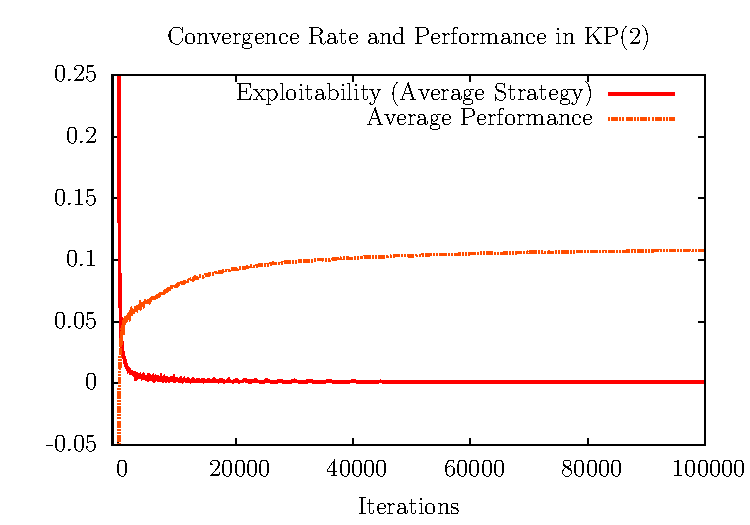
\includegraphics[scale=0.7]{figs/sfrd2-conv} 

\hspace{-0.5cm}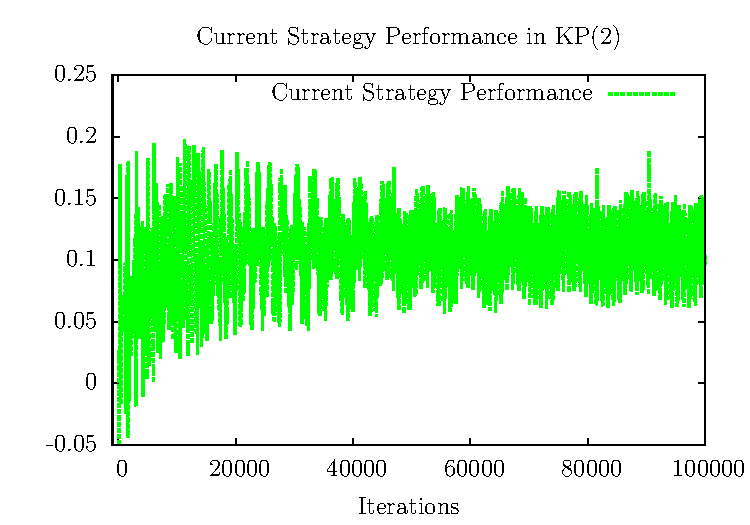
\includegraphics[scale=0.7]{figs/sfrd2-curperf}
\end{center}
\caption{Top: convergence rate and overall performance of average strategy in KP$(2)$. Bottom: overall performance
of the current strategy. In both cases, the vertical axis represents utility. \label{fig:sfrd2-conv}}
\end{figure}

We first analyze the behavior of SFRD in two-player Kuhn poker. 
In two-player zero-sum games, 
a common way to compute distance to an equilibrium is to use exploitability. Since $u_2(\sigma) = -u_1(\sigma)$, 
the gap in Equation~\ref{eq:ne} is replaced by 
$\max_{\sigma_1' \in \Sigma_1} u_1(\sigma_1', \sigma_2) + \max_{\sigma_2' \in \Sigma_2} u_2(\sigma_1, \sigma_2')$. 
Therefore, in the case of two players, the graphs show exploitability. 

The convergence rate and overall performance of the average and current strategy profiles are shown in
Figure~\ref{fig:sfrd2-conv}. The exploitability quickly drops from to low values within the first few hundred iterations. 
The values for $t = (100,200,300)$ are $(0.916, 0.171, 0.096)$ to less than $0.001$ at $t = 100000$. 
The average performance slowly but steadily rises from $-0.25$ initially to $0.109$ at $t = 100000$. The performance of the 
current strategy is much noisier, suggesting that players are switching significantly between alternatives, 
but slowly seems to concentrate to a neighborhood around $0.1$ as well.

\subsection{Multiplayer Experiments}

\begin{figure*}[t]
\begin{center}
\begin{tabular}{cc}
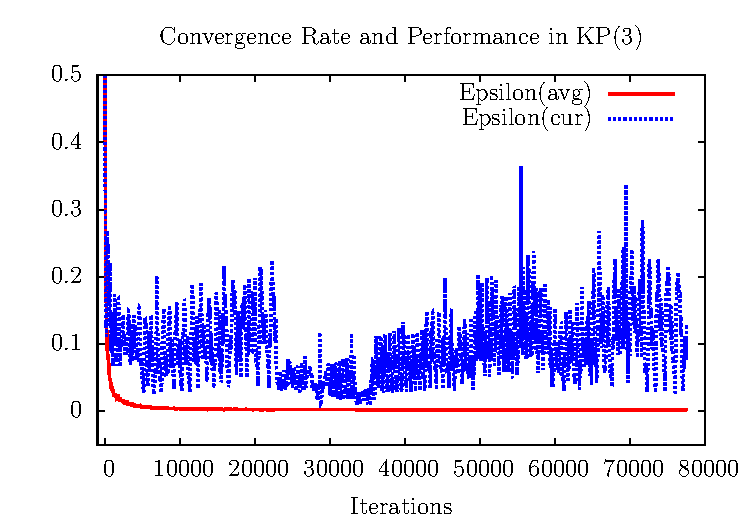
\includegraphics[scale=0.7]{figs/sfrd3-conv}    & 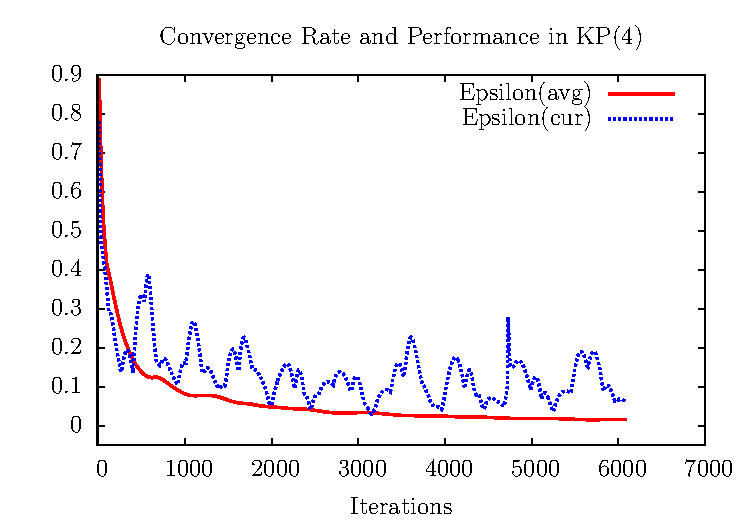
\includegraphics[scale=0.7]{figs/sfrd4-conv} \\
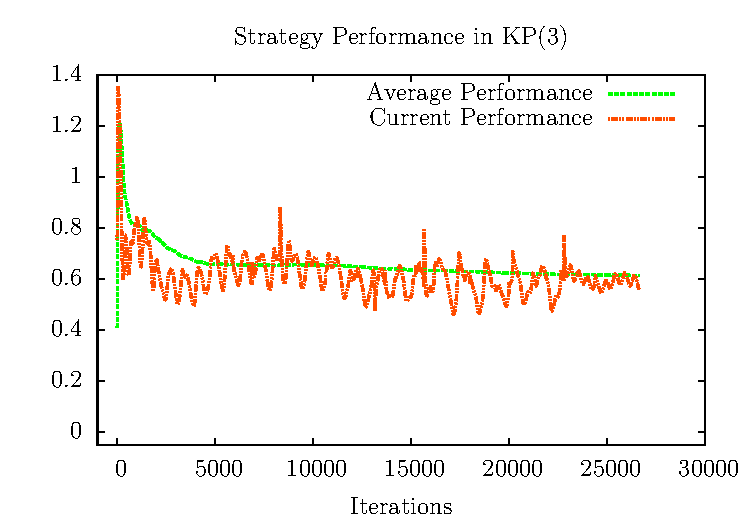
\includegraphics[scale=0.7]{figs/sfrd3-perf}    & 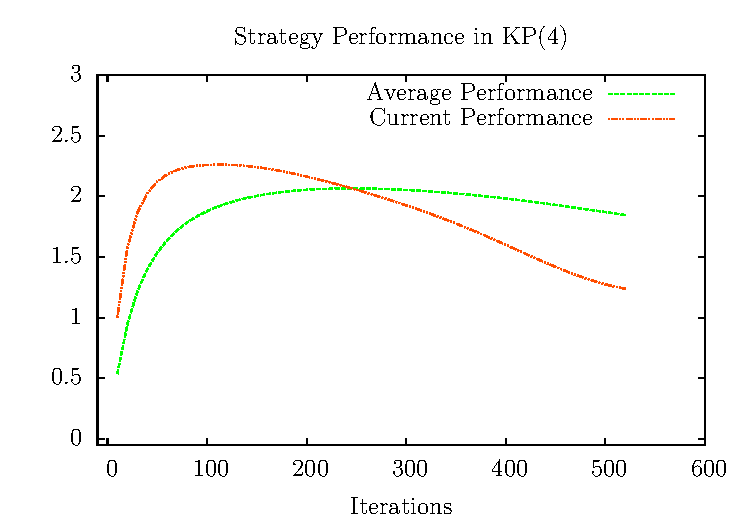
\includegraphics[scale=0.7]{figs/sfrd4-perf} \\
\end{tabular}
\end{center}
\caption{Convergence rate and overall performance in KP$(3)$ (left) and KP$(4)$ (right). 
The vertical axes represent utility. 
Epsilon(avg) and Epsilon(cur) represent the convergence rates
of $\bar{\bx}(t)$ and $\bx(t)$, respectively. \label{fig:sfrd34}}
\end{figure*}

In this section, we present experiments for KP$(3)$ and KP$(4)$.  The convergence rates and performances are shown in 
Figure~\ref{fig:sfrd34}.

In KP$(3)$, we notice that again that $\bar{\bx}(t)$ reaches to a low value of $\epsilon$ relatively quickly, within 
a few thousand iterations, reaching $\epsilon \approx 0.00169$ at $t = 100000$. 
Interstingly, unlike 
the current strategy profile does not seem to be converging closer to a Nash equilibrium. This might indicate that the evolution 
has not found any attracting stable fixed points or that the strategies are ``orbitting'' around a fixed point, possibly the one 
represented by $\bar{\bx}(t)$. 
From the performance graphs, we see that early on the performance spikes and 
and then slowly decreases. This could be due the players cooperating to increase the score against the early 
strategies close to the baseline, which slowly decreases as each player learns to counter the opponents, 
eventually stabalizing around $0.615$. The current strategy
performance graph is noisy as in KP$(2)$, and the performance of the average strategy seems to be higher at first ($t \le 30000$). 

In KP$(4)$, again the average profile seems to be reducing $\epsilon$ smoothly and getting closer to a Nash equilibrium 
over time, reaching $\epsilon \approx 0.033$ at $t = 2980$. 
Like in KP$(3)$, the $\epsilon$ convergence of the current strategies $\bx(t)$ is erratic. 
As in KP$(4)$, the performance of the current strategy is seems less than the average 
strategy $\bar{\bx}(t)$, which is consistent with the KP$(3)$ results. 

In all cases, the average strategy profile $\bar{\bx}$ seems to be converging to equilibrium with $\epsilon$ decreasing as the
number of iterations increase. 
While convergence is guaranteed in two-player no-regret learning, the results here suggest this may also hold in SFRD with 
any number of players.  
Also, since the dynamics are realization-equivalent to standard replicator dynamics, dominated strategies will not survive 
in the current strategies and will slowly be played less and less in the average strategies as well. 
In all cases, both current and average strategy seems better than the baseline, but the average strategies sometimes perform 
better and appear to be more stable in time. 

\section{Conclusion}

\todo{conclude!}


%ACKNOWLEDGMENTS are optional
%\section{Acknowledgments}
%This section is optional; it is a location for you
%to acknowledge grants, funding, editing assistance and
%what have you.  In the present case, for example, the
%authors would like to thank Gerald Murray of ACM for
%his help in codifying this \textit{Author's Guide}
%and the \textbf{.cls} and \textbf{.tex} files that it describes.

%
% The following two commands are all you need in the
% initial runs of your .tex file to
% produce the bibliography for the citations in your paper.
\bibliographystyle{abbrv}
\bibliography{sfegt}  % sigproc.bib is the name of the Bibliography in this case
% You must have a proper ".bib" file
%  and remember to run:
% latex bibtex latex latex
% to resolve all references
%
% ACM needs 'a single self-contained file'!
%
%APPENDICES are optional
%\balancecolumns
%\appendix
%Appendix A
\end{document}
